\documentclass[a4paper]{article}%字号5号
\usepackage{natbib}
\setcitestyle {numbers,square}
\usepackage{xpatch}
\ExplSyntaxOn
\makeatletter
\xpatchcmd{\@maketitle}
{
    \@title
}
{
    \heiti\zihao{3}\@title
}
{}{\fail}
\xpatchcmd{\@maketitle}
{
    \@author
}
{
    \kaishu\zihao{-4}\@author
}
{}{\fail}
\makeatother
\ExplSyntaxOff
\usepackage{ctex}%输出汉字
\usepackage{times}%英文字体

\title{虹与霓}%黑体三号,行距1.5倍
%%\author{范潇\phantom{1}陈思同\phantom{1}吴靖阳}%小四字号,1.5倍行距,仿宋
\author{范潇\phantom{1}刘嘉程}
\date{}%去除日期
\linespread{1.5}%行间距1.5倍
\usepackage{amsmath,amsthm,amssymb,graphicx}
\usepackage[]{pifont}
\usepackage{float}
\usepackage{caption}
\usepackage{unicode-math}
\usepackage{setspace}
\usepackage{subfigure}
\usepackage[export]{adjustbox}%防止过宽的图片
\usepackage{bibentry,natbib}%两个参考文献宏包
\usepackage{abstract}
\usepackage{fontspec}
\usepackage{xeCJK}
\setCJKmainfont{SimSun}
\setCJKsansfont{SimSun}
\setCJKmonofont{SimSun}%正文字体为宋体
\usepackage[fontsize=10.5pt]{fontsize}
\renewcommand{\abstracttextfont}{\fangsong}%摘要字体改为仿宋
\renewcommand{\abstractname}{\textbf{摘\quad 要}}%更改摘要两字的样式
\usepackage{indentfirst}%中文首行缩进
\usepackage[left=2.50cm,right=2.50cm,top=2.80cm,bottom=2.50cm]{geometry}%页边距设置
\bibliographystyle{unsrt}%让引用序号按照顺序排列
\newtheorem{thm}{定理}
\newtheorem{definiton}{定义}
\newcommand*\abs[1]{\lvert#1\rvert}%绝对值符号
\newcommand\Emph{\textbf}%粗体强调命令
\usepackage{indentfirst}
\usepackage{makecell}
\usepackage{tabularx}
\begin{document}
  \maketitle  
\begin{abstract}
   彩虹,简称虹,是气象中的一种光学现象,太阳光照射到半空中的水滴,光线被折射及反射,在天空上形成拱形的七彩光谱,由外圈至内圈呈红、橙、黄、绿、蓝、靛、紫.
   霓是经常出现在主虹外侧昏暗的第二道彩虹.霓是阳光经由雨滴内两次反射和两次折射产生的.两次反射的结果,使得霓的色彩排列和虹的弧相反,蓝色在外而红色在内.霓比虹暗弱,因为两次反射不仅使得更多的光线逃逸掉,也使得散布的区域也更为宽广.
   本文试用牛顿和笛卡尔的方法来解释虹和霓的形状、位置和颜色.
\end{abstract}

\section{虹和霓的形状和位置}
%%插入图片一,标题为“虹的形成”
\begin{figure}[ht]
   \centering
   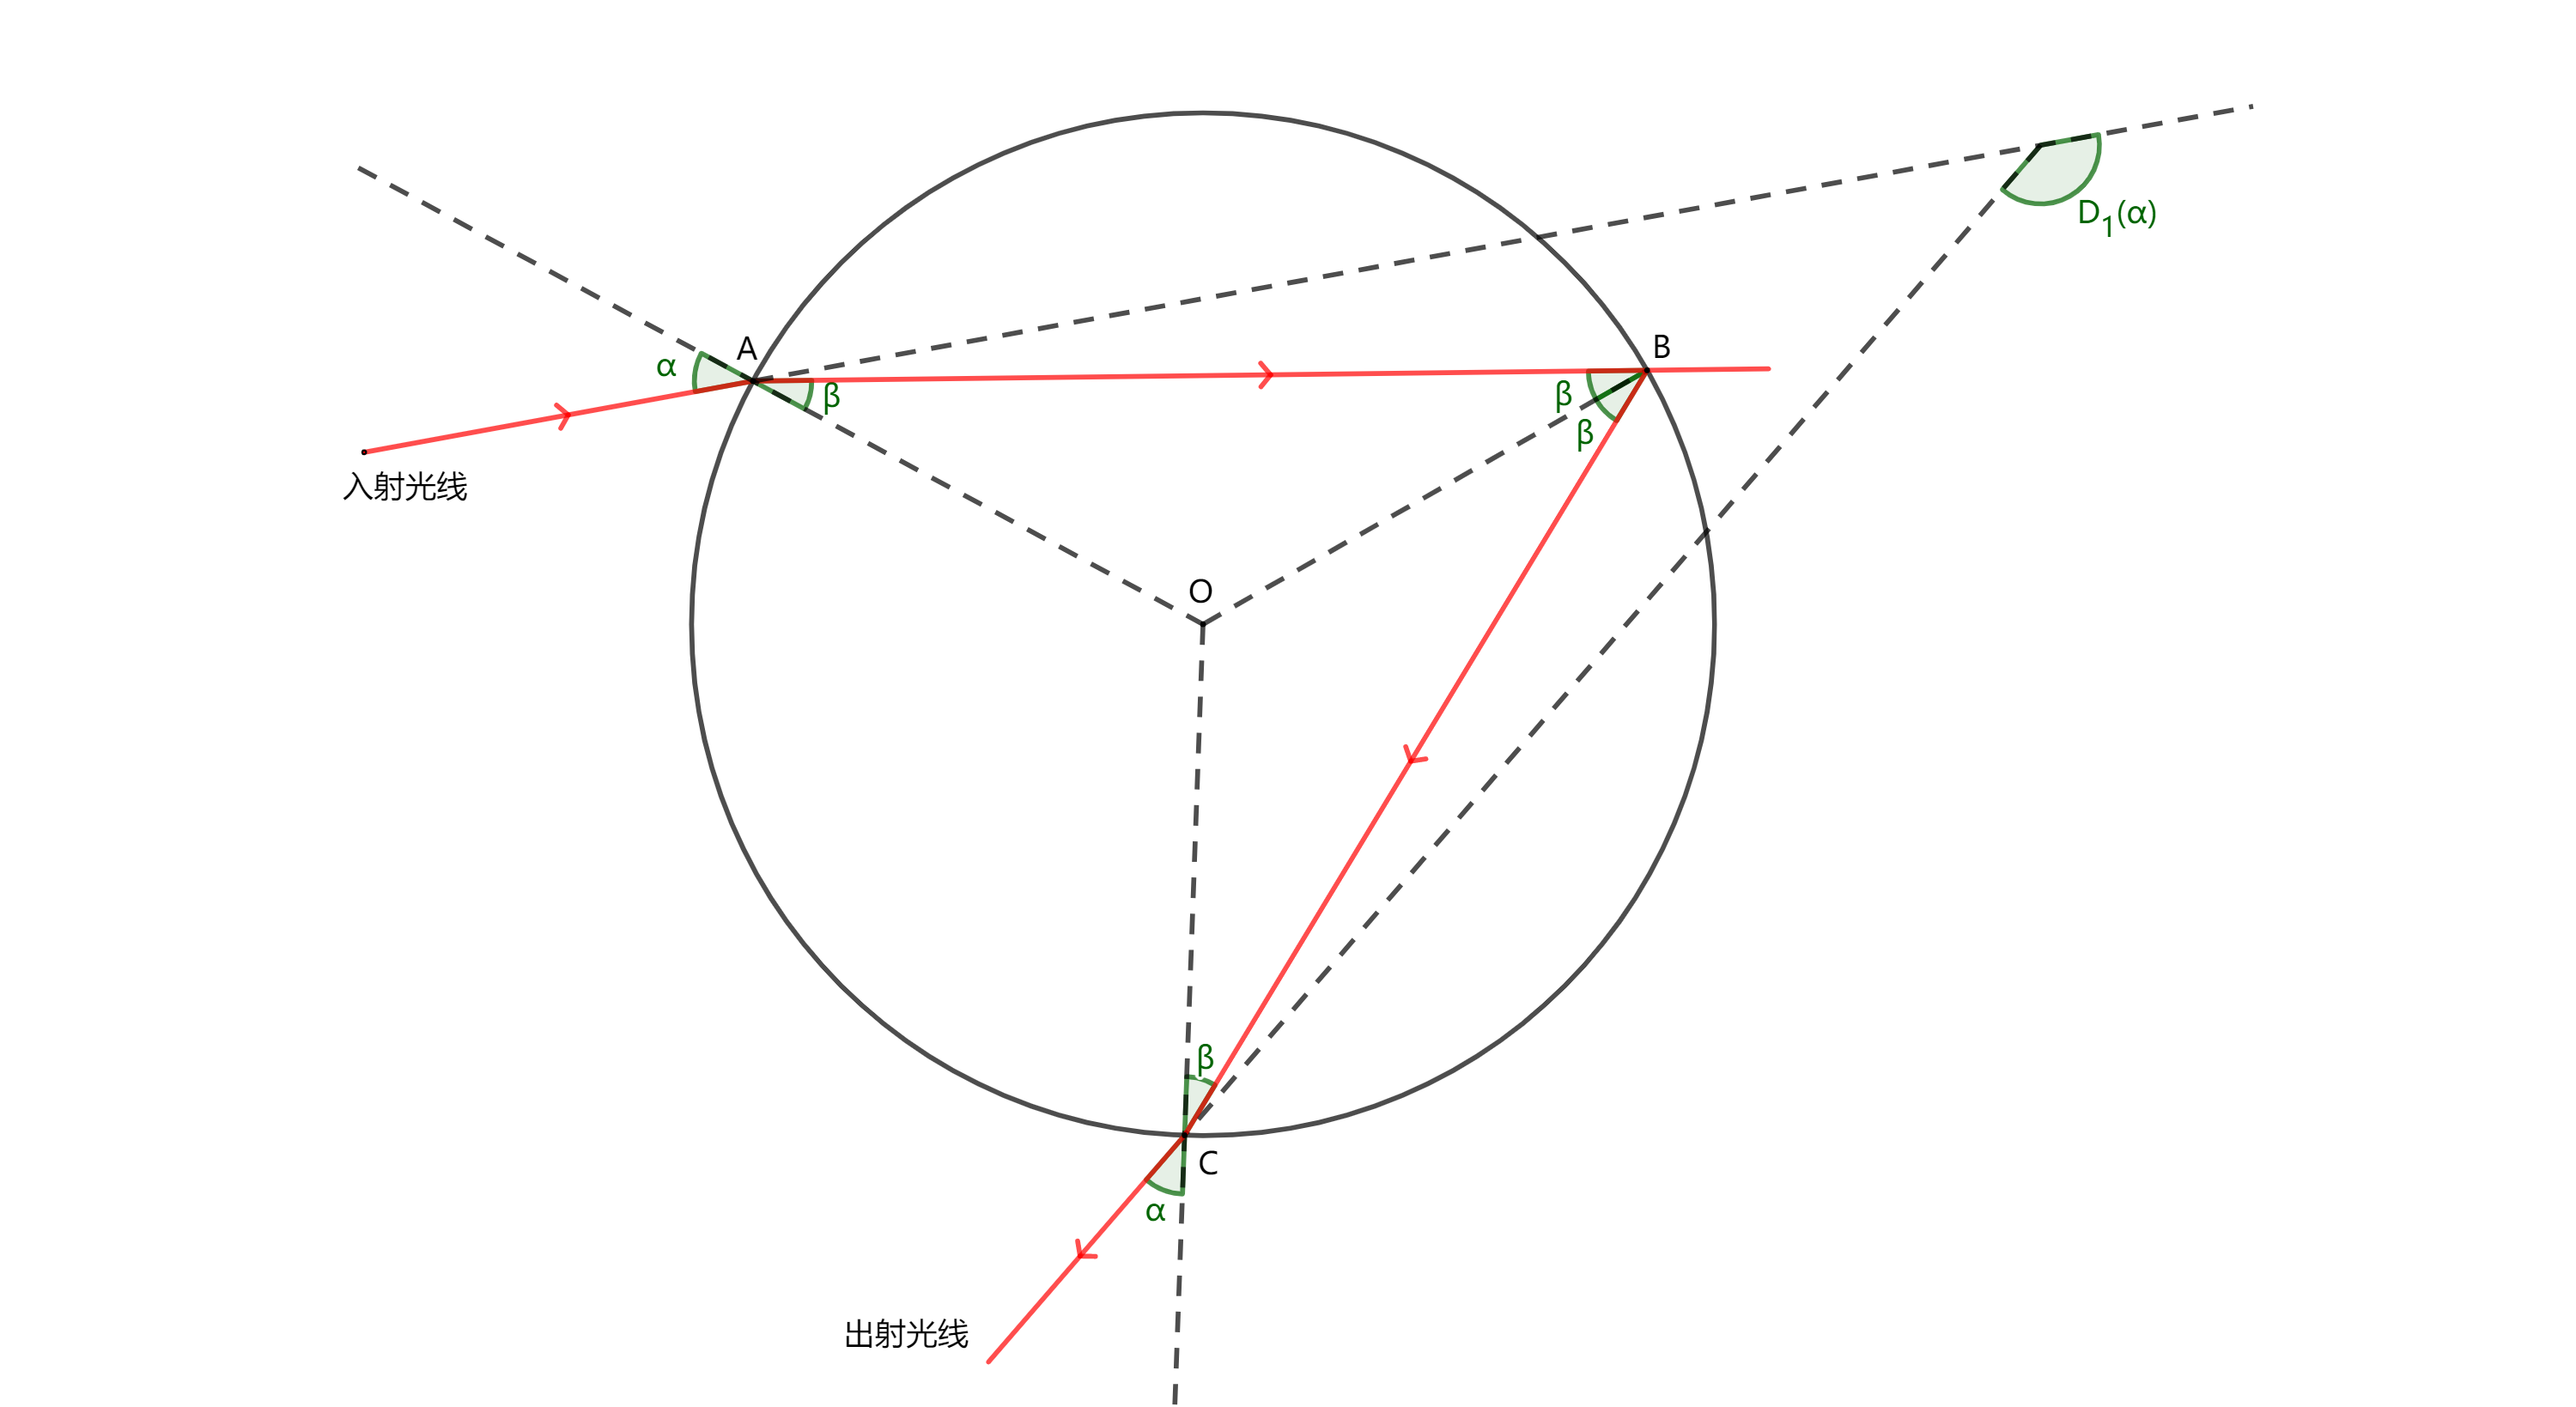
\includegraphics[scale=0.8]{图1}
   \caption[图1]{虹的形成}\label{fig-图1}
   \end{figure}
图1所展示的是一束太阳光在点A折射进入球型雨珠,然后大部分光线在点B反射,最终从点C折射出去这一过程的光路图,其中$\alpha$为入射角,$\beta$为折射角.我们称经过这一过程的出射光线所形成的彩虹为虹.
$D_1(\alpha)$是出射光线方向相比于入射光线方向顺时针偏转的角度.


由几何关系可知,顺时针偏转角
\begin{equation*}
D_1(\alpha)=(\alpha-\beta)+(\pi-2\beta)+(\alpha-\beta)=\pi+2\alpha-4\beta\tag{式1}
\end{equation*}
%%式1
等式两边同时对$\alpha$求导可得
\begin{equation*}
\frac{dD_1}{d\alpha}=2-4\frac{d\beta}{d\alpha}\tag{式2}
\end{equation*}
%%式2
由斯涅尔定律可知
\begin{equation*}
\sin\alpha=k\sin\beta\tag{式3}
\end{equation*}
其中k为折射系数.


%%式3
等式两边同时对$\alpha$求导可得
\[\cos\alpha=k\frac{d\sin\beta}{d\alpha},\]
又因为
\[\frac{d\sin\beta}{d\alpha}=\cos\beta\frac{d\beta}{d\alpha},\]
所以
\begin{equation*}
\frac{d\beta}{d\alpha}=\frac{\cos\alpha}{k\cos\beta}\tag{式4}
\end{equation*}
%%式4
将式4代入式2可得
\begin{equation*}
D_1^{\prime}(\alpha)=2-\frac{4\cos\alpha}{k\cos\beta}\tag{式5}
\end{equation*}
%%式5
令$D_1^{\prime}(\alpha)=0$,则$2\cos\alpha=k\cos\beta$
与式3联立后可得
\[\alpha=\arccos\sqrt\frac{k^2-1}{3},\]
\[\beta=\arccos\sqrt\frac{4k^2-4}{3k^2},\]
因为顺时针偏转角最小值客观存在,而当$D_1^{\prime}(\alpha)=0$时,在$(0,\pi/2)$内$\alpha$只有唯一解
\[\alpha=\arccos\sqrt\frac{k^2-1}{3},\]
所以当$\alpha$取此值时,顺时针偏转角$D_1(\alpha)$取得最小值
\[D_{1\min}=\pi+2\arccos\sqrt\frac{k^2-1}{3}-4\arccos\sqrt\frac{4k^2-4}{3k^2},\]
此时$\Delta D_1/\Delta\alpha\approx 0$,这意味着大量入射角$\alpha\approx \arccos\sqrt {(k^2-1)/3}$的太阳光线的偏转程度近乎相同.
正是这种在最小偏转角附近所产生的光线聚集的现象使得虹变得明亮.
我们把观察者与彩虹最高点处的连线与太阳光方向所成的锐角称为彩虹角.
%%插入图片2.标题为:彩虹角与顺时针偏转角的关系
\begin{figure}[ht]
   \centering
   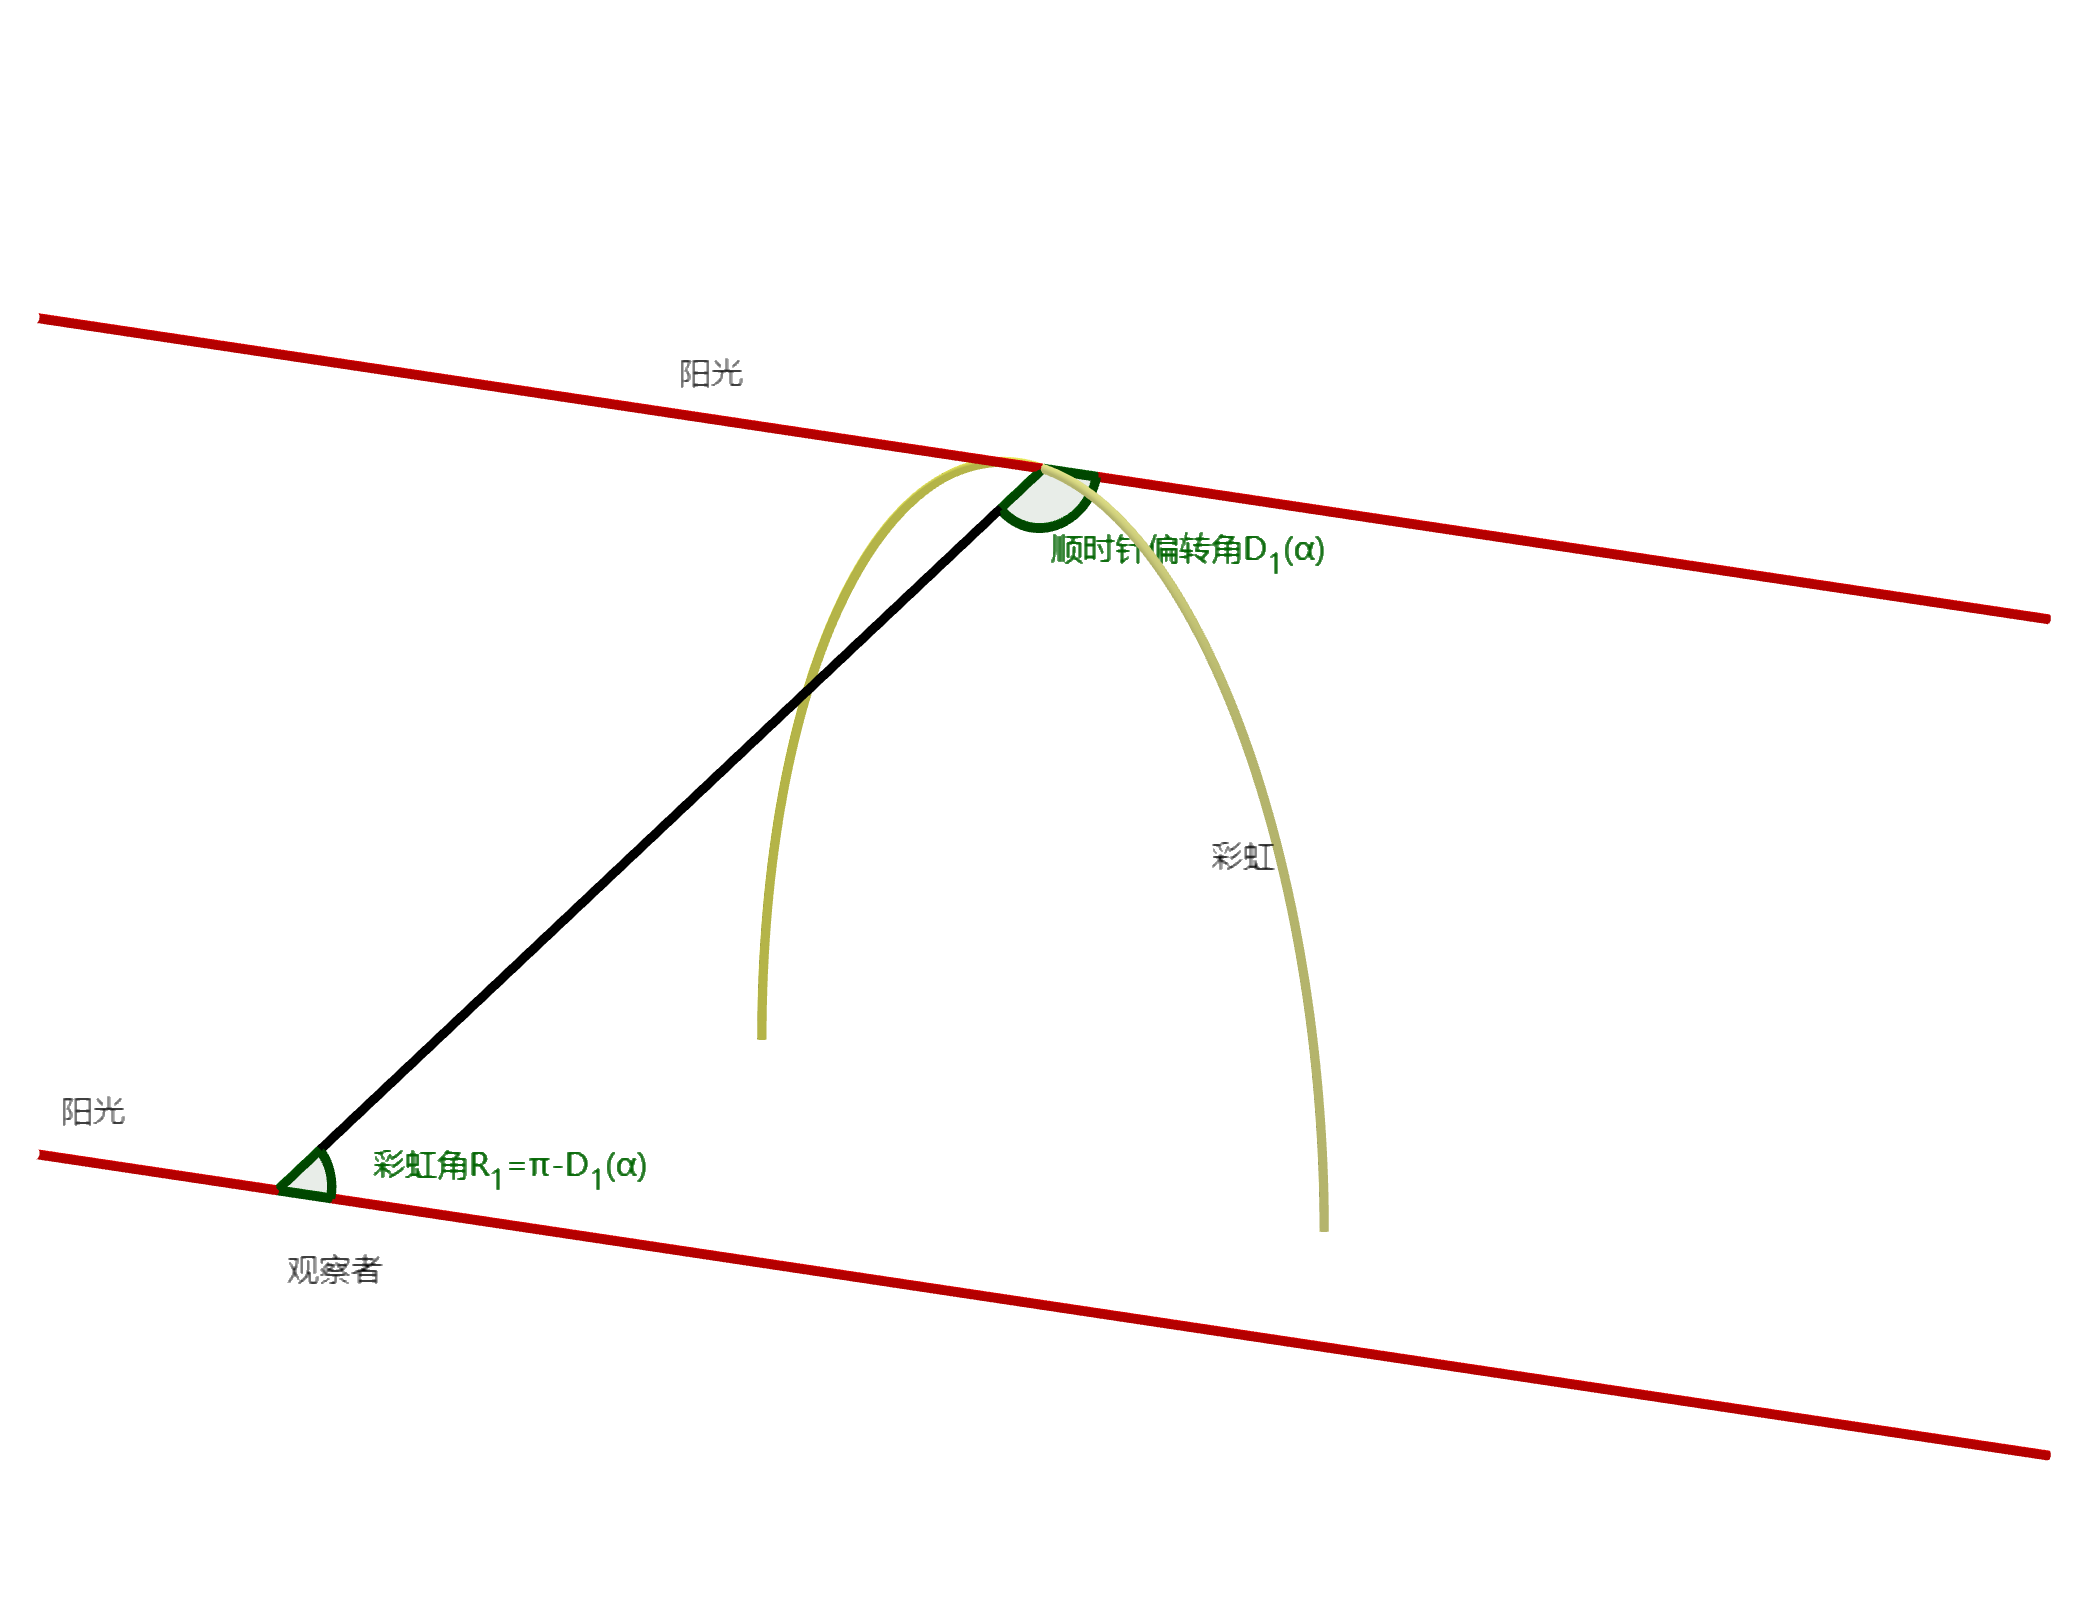
\includegraphics[scale=0.14]{图2}
   \caption[图2]{彩虹角与顺时针偏转角的关系}\label{fig-图2}
   \end{figure}


此时的彩虹角
\[R_1(k)=\pi-D_{1\min}=4\arccos\sqrt\frac{4k^2-4}{3k^2}-2\arccos\sqrt\frac{k^2-1}{3}.\]
对于固定的$k$,彩虹角$R_1$为定值,因此我们所看到的彩虹是由一层层色环所组成的.

%插入图片3:霓的形成
\begin{figure}[H]
   \centering
   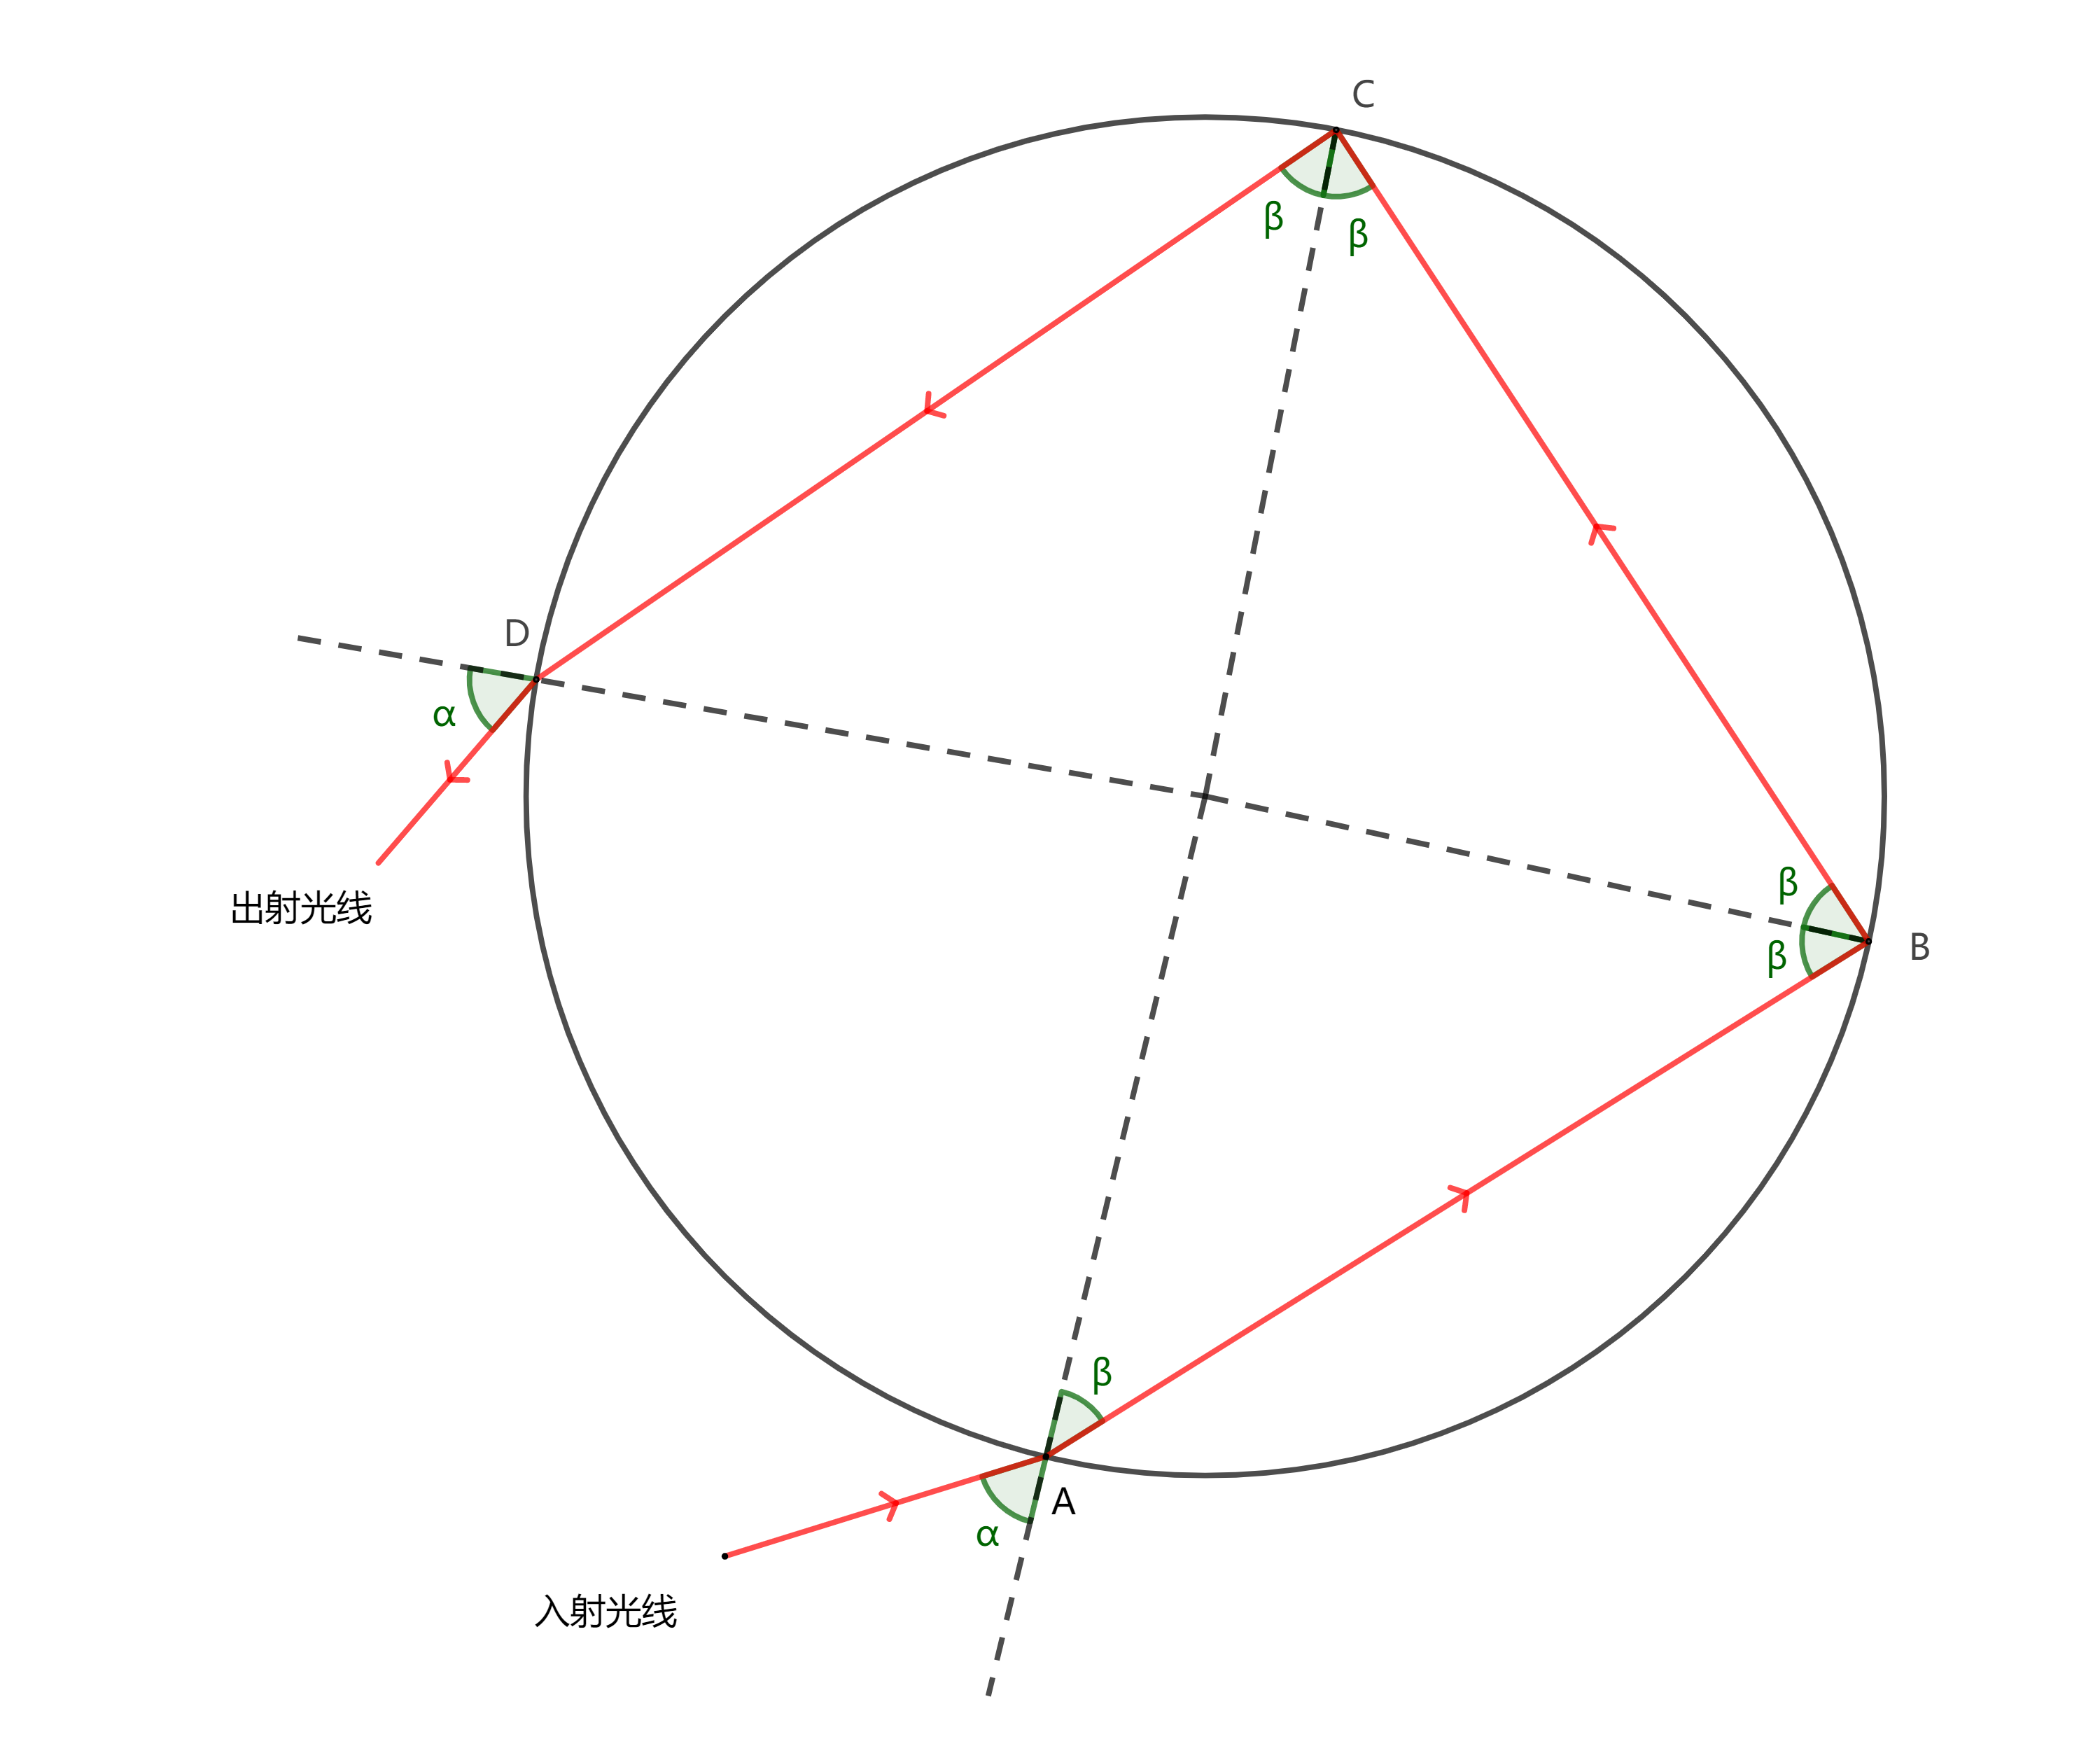
\includegraphics[scale=0.75]{图3}
   \caption[图3]{霓的形成}\label{fig-图3}
   \end{figure}


图3所展示的是一束太阳光在点A折射进入球型雨珠,然后依次在点B、点C处反射,最终从点D折射出去这一过程的光路图,其中$\alpha$为入射角,$\beta$为折射角.
值得注意的是,这4次折(反)射使得光线的能量有了较为明显的损失.我们称经过这一过程的出射光线所形成的彩虹为霓.



记$D_2(\alpha)$为出射光线方向相比于入射光线方向逆时针偏转的角度.


由几何关系可得,逆时针偏转角
\[D_2(\alpha)=2\alpha-6\beta+2\pi,\]
重复第一种情况的计算可得
当$\alpha=\arccos\sqrt{(k^2-1)/8}$时,逆时针偏转角$D_2(\alpha)$取得最小值
\[D_{2\min}=2\arccos\sqrt\frac{k^2-1}{8}-6\arccos\sqrt\frac{9k^2-9}{8k^2}+2\pi,\]
此时的彩虹角
\[R_2(k)=D_{2\min}-\pi=2\arccos\sqrt\frac{k^2-1}{8}-6\arccos\sqrt\frac{9k^2-9}{8k^2}+\pi.\]
%%插入图片4标题为:彩虹角与逆时针偏转角的关系
\begin{figure}[ht]
   \centering
   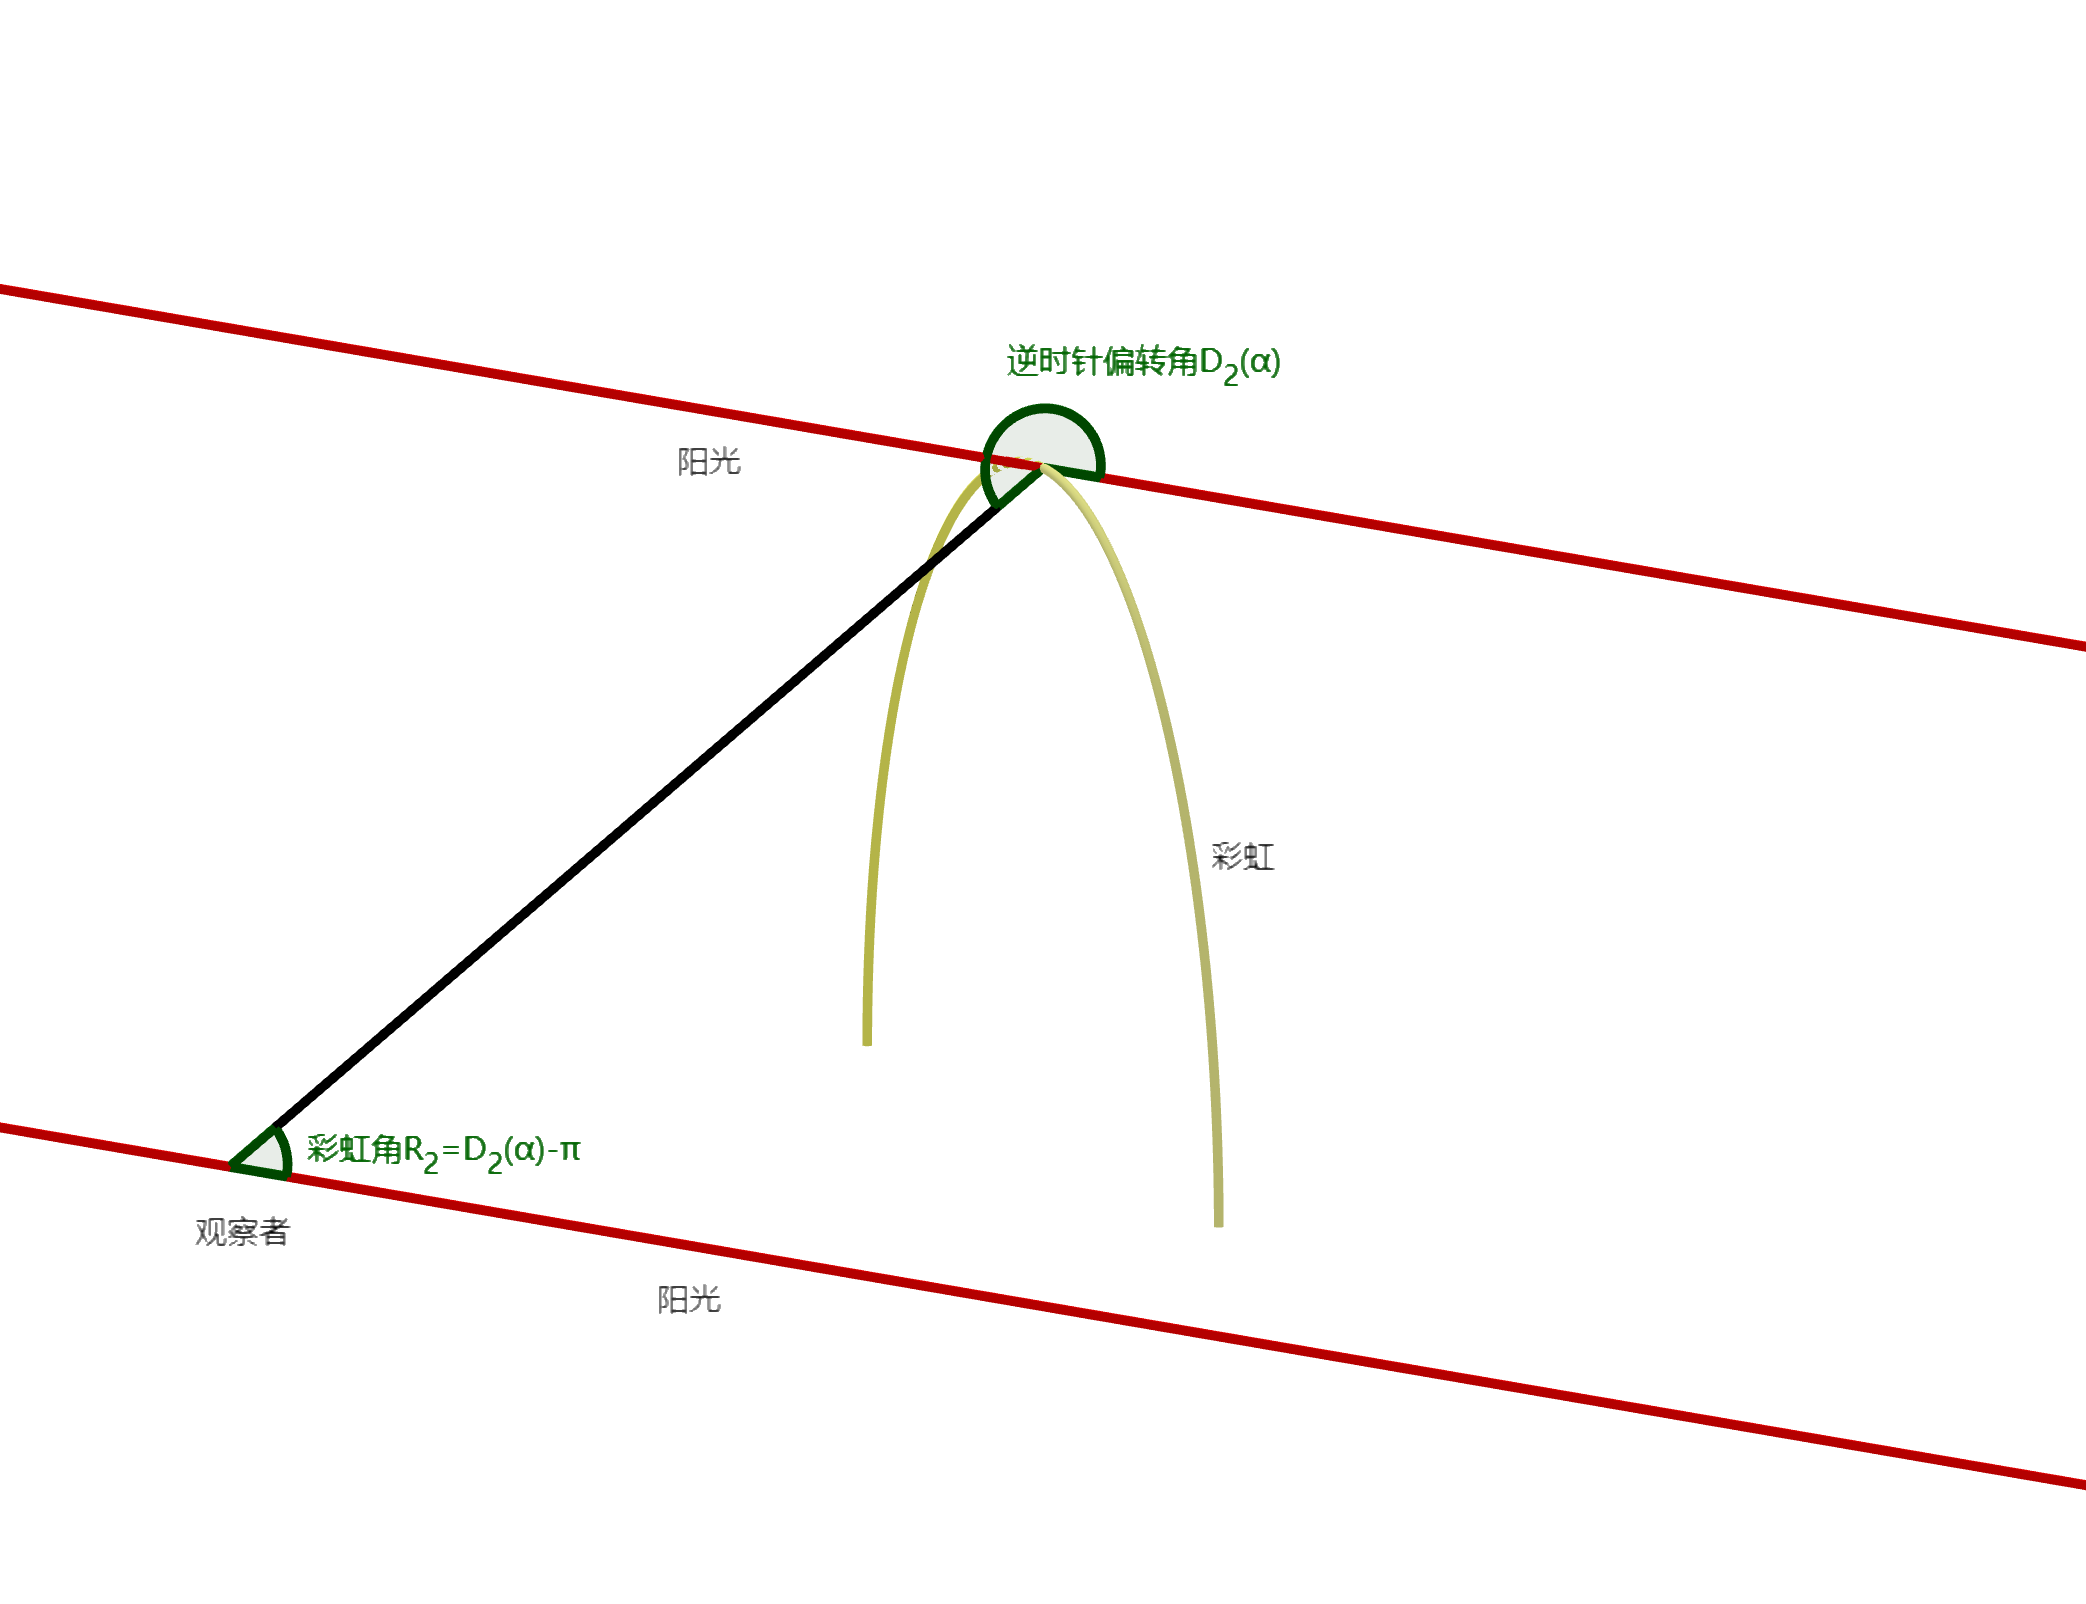
\includegraphics[scale=0.14]{图4}
   \caption[图4]{彩虹角与逆时针偏转角的关系}\label{fig-图4}
   \end{figure}
   \\
特别地,取$k=\frac{4}{3}$(水的折射系数),
当$\alpha\approx 59.4^{\circ }$时,
\[D_1=D_{1\min}\approx 138^{\circ },R_1\approx 42^{\circ }.\]
当$\alpha\approx 71.8^{\circ }$时,
\[D_2=D_{2\min}\approx 231^{\circ },R_2\approx 51^{\circ }.\]
这也就意味着,从地面上去看,霓总是在虹上方.并且由于霓是阳光经过四次折(反)射形成的,比只经过三次折(反)射就形成的虹损失的能量更多,所以后者比前者看起来更加清晰.
%%插入图片1542495,虹和霓的相对位置
\begin{figure}[ht]
   \centering
   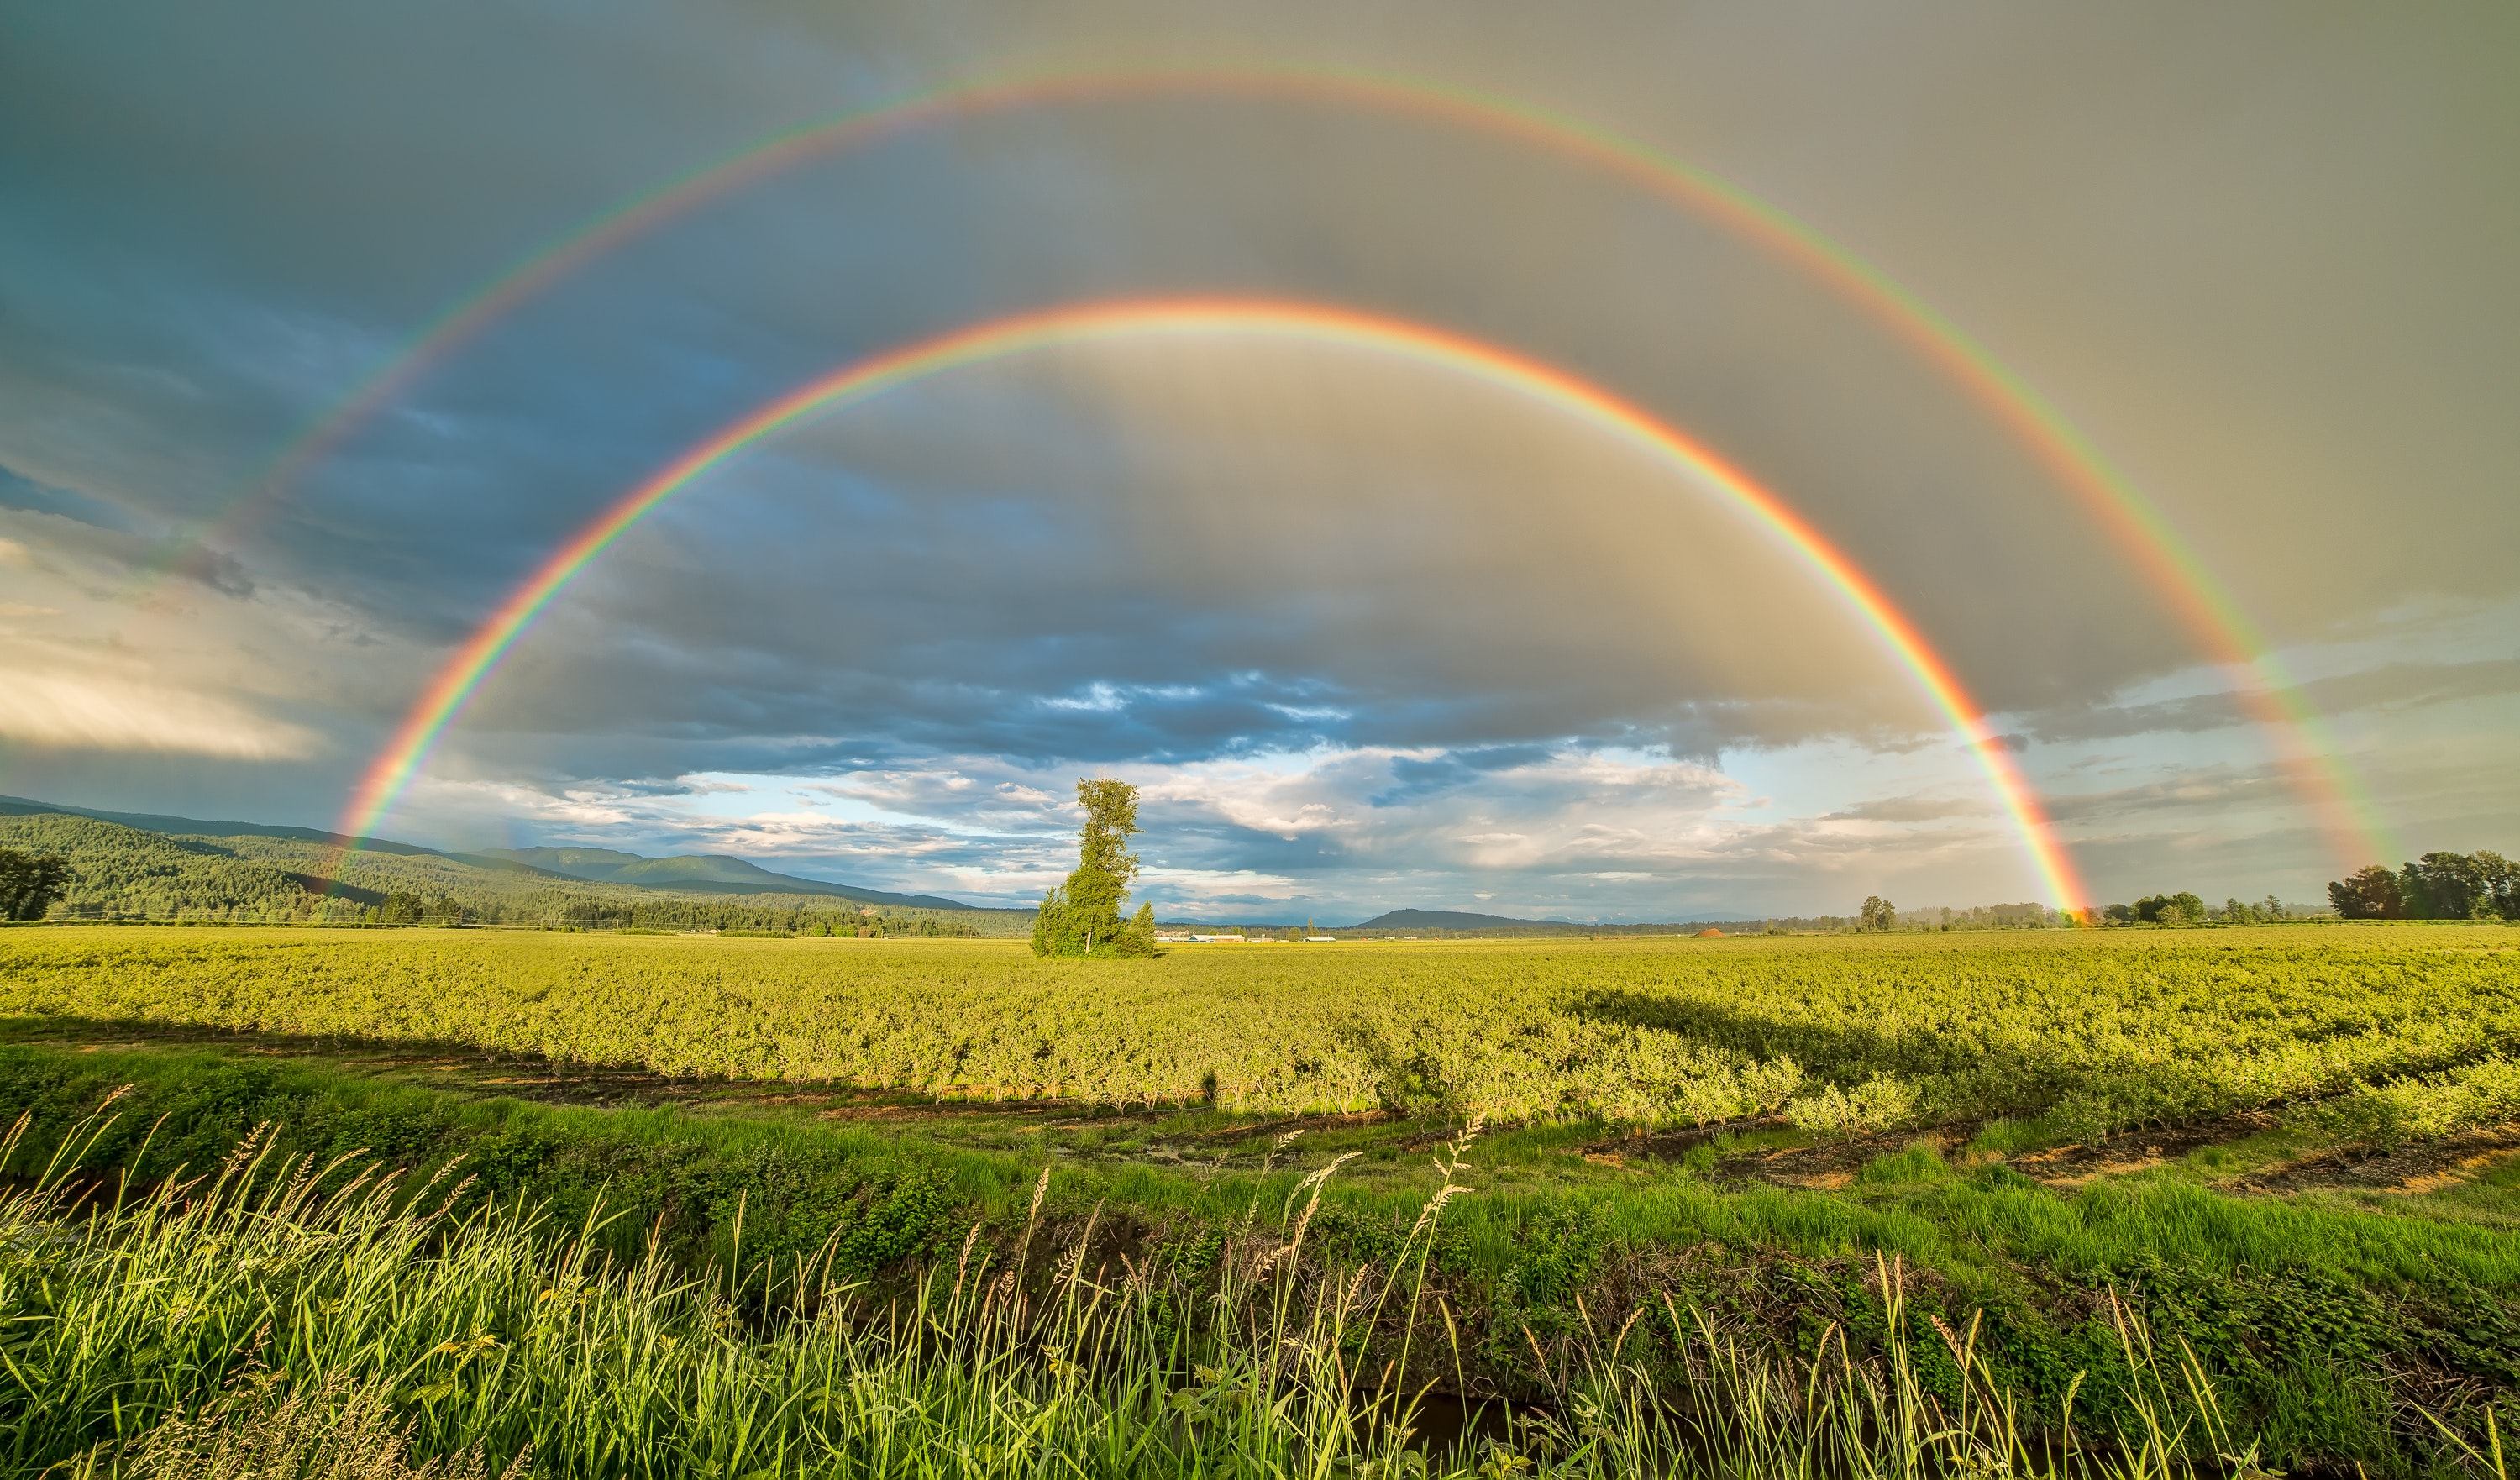
\includegraphics[scale=0.12]{图5}
   \caption[图5]{虹和霓的相对位置}\label{fig-图5}
   \end{figure}
\section{虹和霓的颜色}
彩虹中的七色光的波长分布在380-700nm中,而不同波长的光在蒸馏水中的折射系数k不同.
Masahiko Daimon和Akira Masumura测量了波长不同的光在蒸馏水中的折射系数,
根据表1与表2的数据,本文中折射系数$k$的取值范围为1.33-1.35.
%%表格形式,标题为波长不同的光在蒸馏水中20℃时的折射系数

\begin{table}[ht]
   \begin{minipage}{0.48\linewidth}
   \centering
   \caption{七色光的波长范围}
\begin{tabular}{|c|c|}
   \hline
   \thead{颜色}&
   \thead{波长范围(nm)}\\ \hline
   红光&625-700\\
橙光&590-625\\
黄光&565-590\\
绿光&500-565\\
靛光&485-500\\
蓝光&450-485\\
紫光&380-450\\
   \hline 
   \end{tabular}
\end{minipage}\begin{minipage}{0.48\linewidth}
\centering
\caption{波长不同的光在蒸馏水中20℃时的折射系数\cite{a}}
\begin{tabular}{|c|c|} 
   \hline  
   \thead{波长(nm)}&
   \thead{折射系数}\\ \hline
   706.714&1.330376\\
   656.454&1.331509\\
   644.025&1.331817\\
   587.725&1.333399\\
   546.227&1.334825\\
   486.269&1.337485\\
   480.126&1.337811\\
   435.957&1.340578\\
   404.770&1.343113\\
   365.119&1.347400\\  
   \hline
   \end{tabular}
\end{minipage}
\end{table}
当$k\in(1.33,1.35)$时,$R_1(k)$严格单调递减,$R_2(k)$严格单调递增,而折射系数k和光波长呈单调关系.
这也就意味着人们抬头看到的虹和霓从下到上的颜色顺序是相反的,分别是由紫到红和由红到紫.同时,由表3可知,霓散布的范围更为宽广,这进一步使得霓看起来比虹更加昏暗.


%%表格形式,标题为七色光的臂长范围
%%插入“彩虹角(角度制)-折射系数图”

%%表格标题:虹和霓中红光光带和紫光光带的彩虹角
\begin{center}\begin{table}[tp]
   \centering
   \caption{虹和霓中红光光带和紫光光带的彩虹角}
   \begin{tabular}{|c|c|c|c|}
      \hline
      \thead{折射系数}&
      \thead{颜色}&
      \thead{$R_1$}&
      \thead{$R_2$}\\ \hline
      1.3318 & 红色 & $42.3^{\circ }$ & $50.6^{\circ }$ \\
      1.3435 & 紫色 & $40.6^{\circ }$ & $53.6^{\circ }$ \\
      \hline
      \end{tabular}
   \end{table}
\end{center}
 
  %%插入彩虹图片2279334,虹和霓的颜色与亮度
\begin{figure}[H]
   \centering
   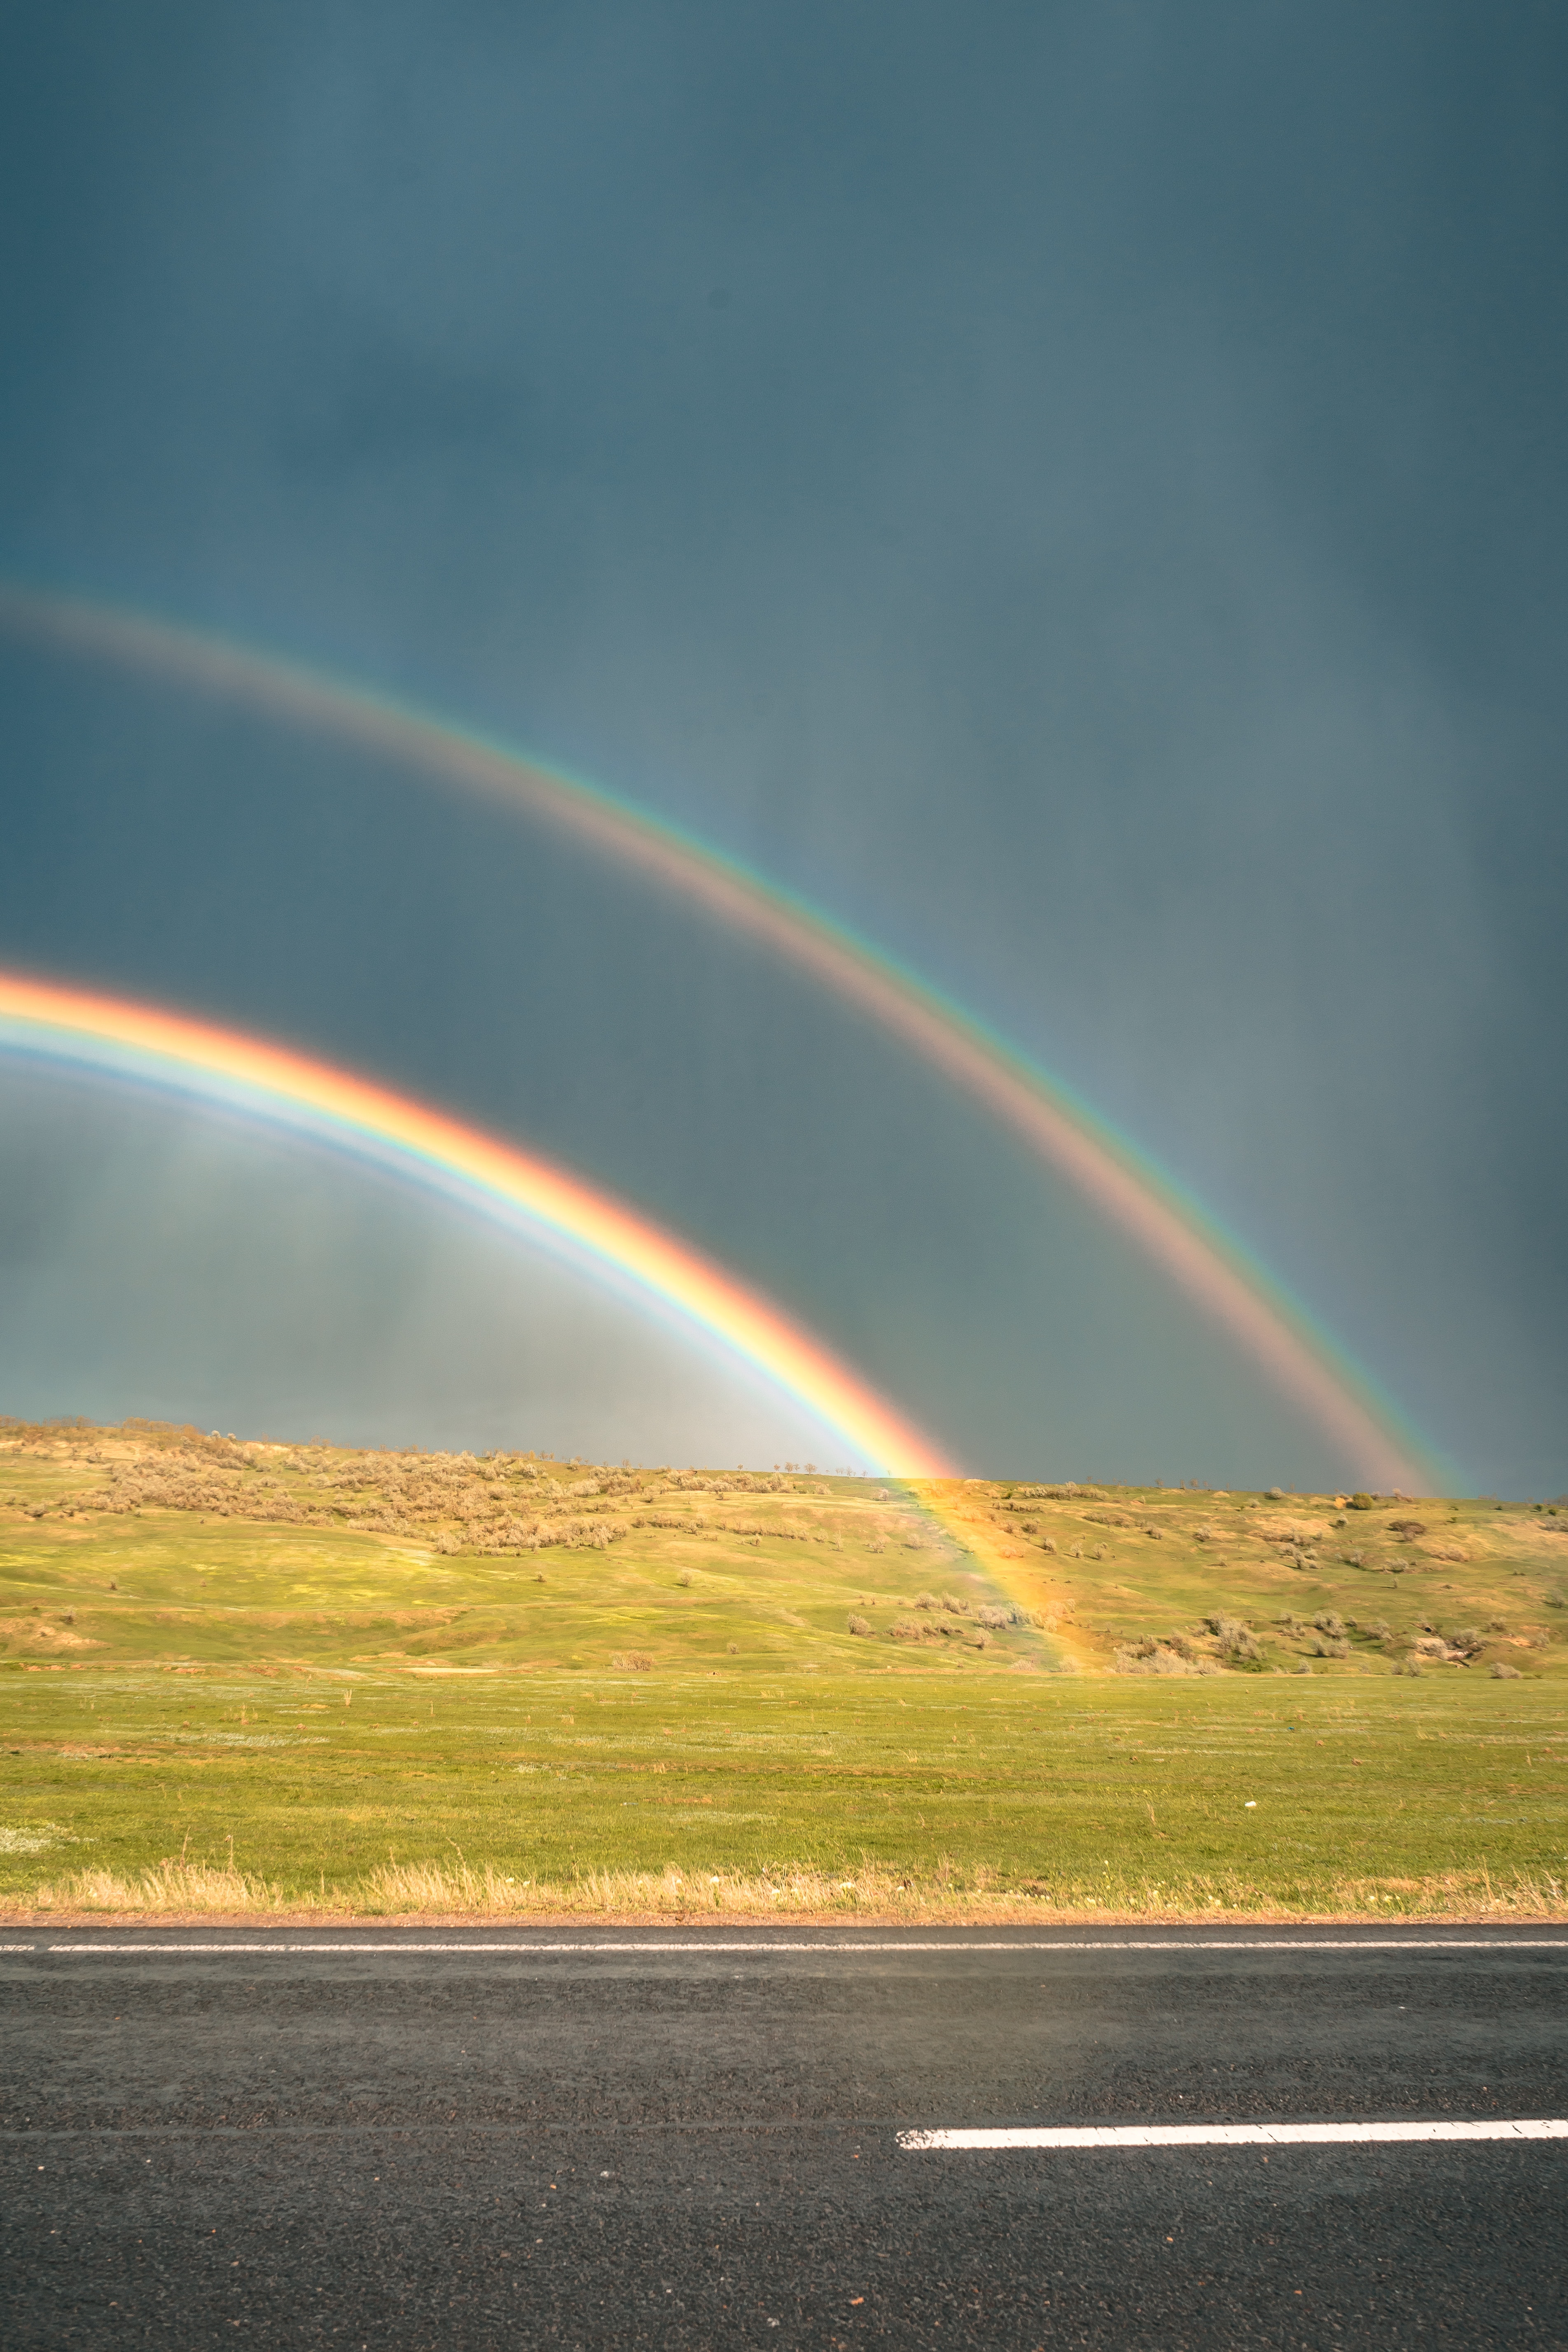
\includegraphics[scale=0.09]{图7}
   \caption[图7]{虹和霓的颜色与亮度}\label{fig-图7}
   \end{figure}
     \begin{figure}[tp]
   \centering
   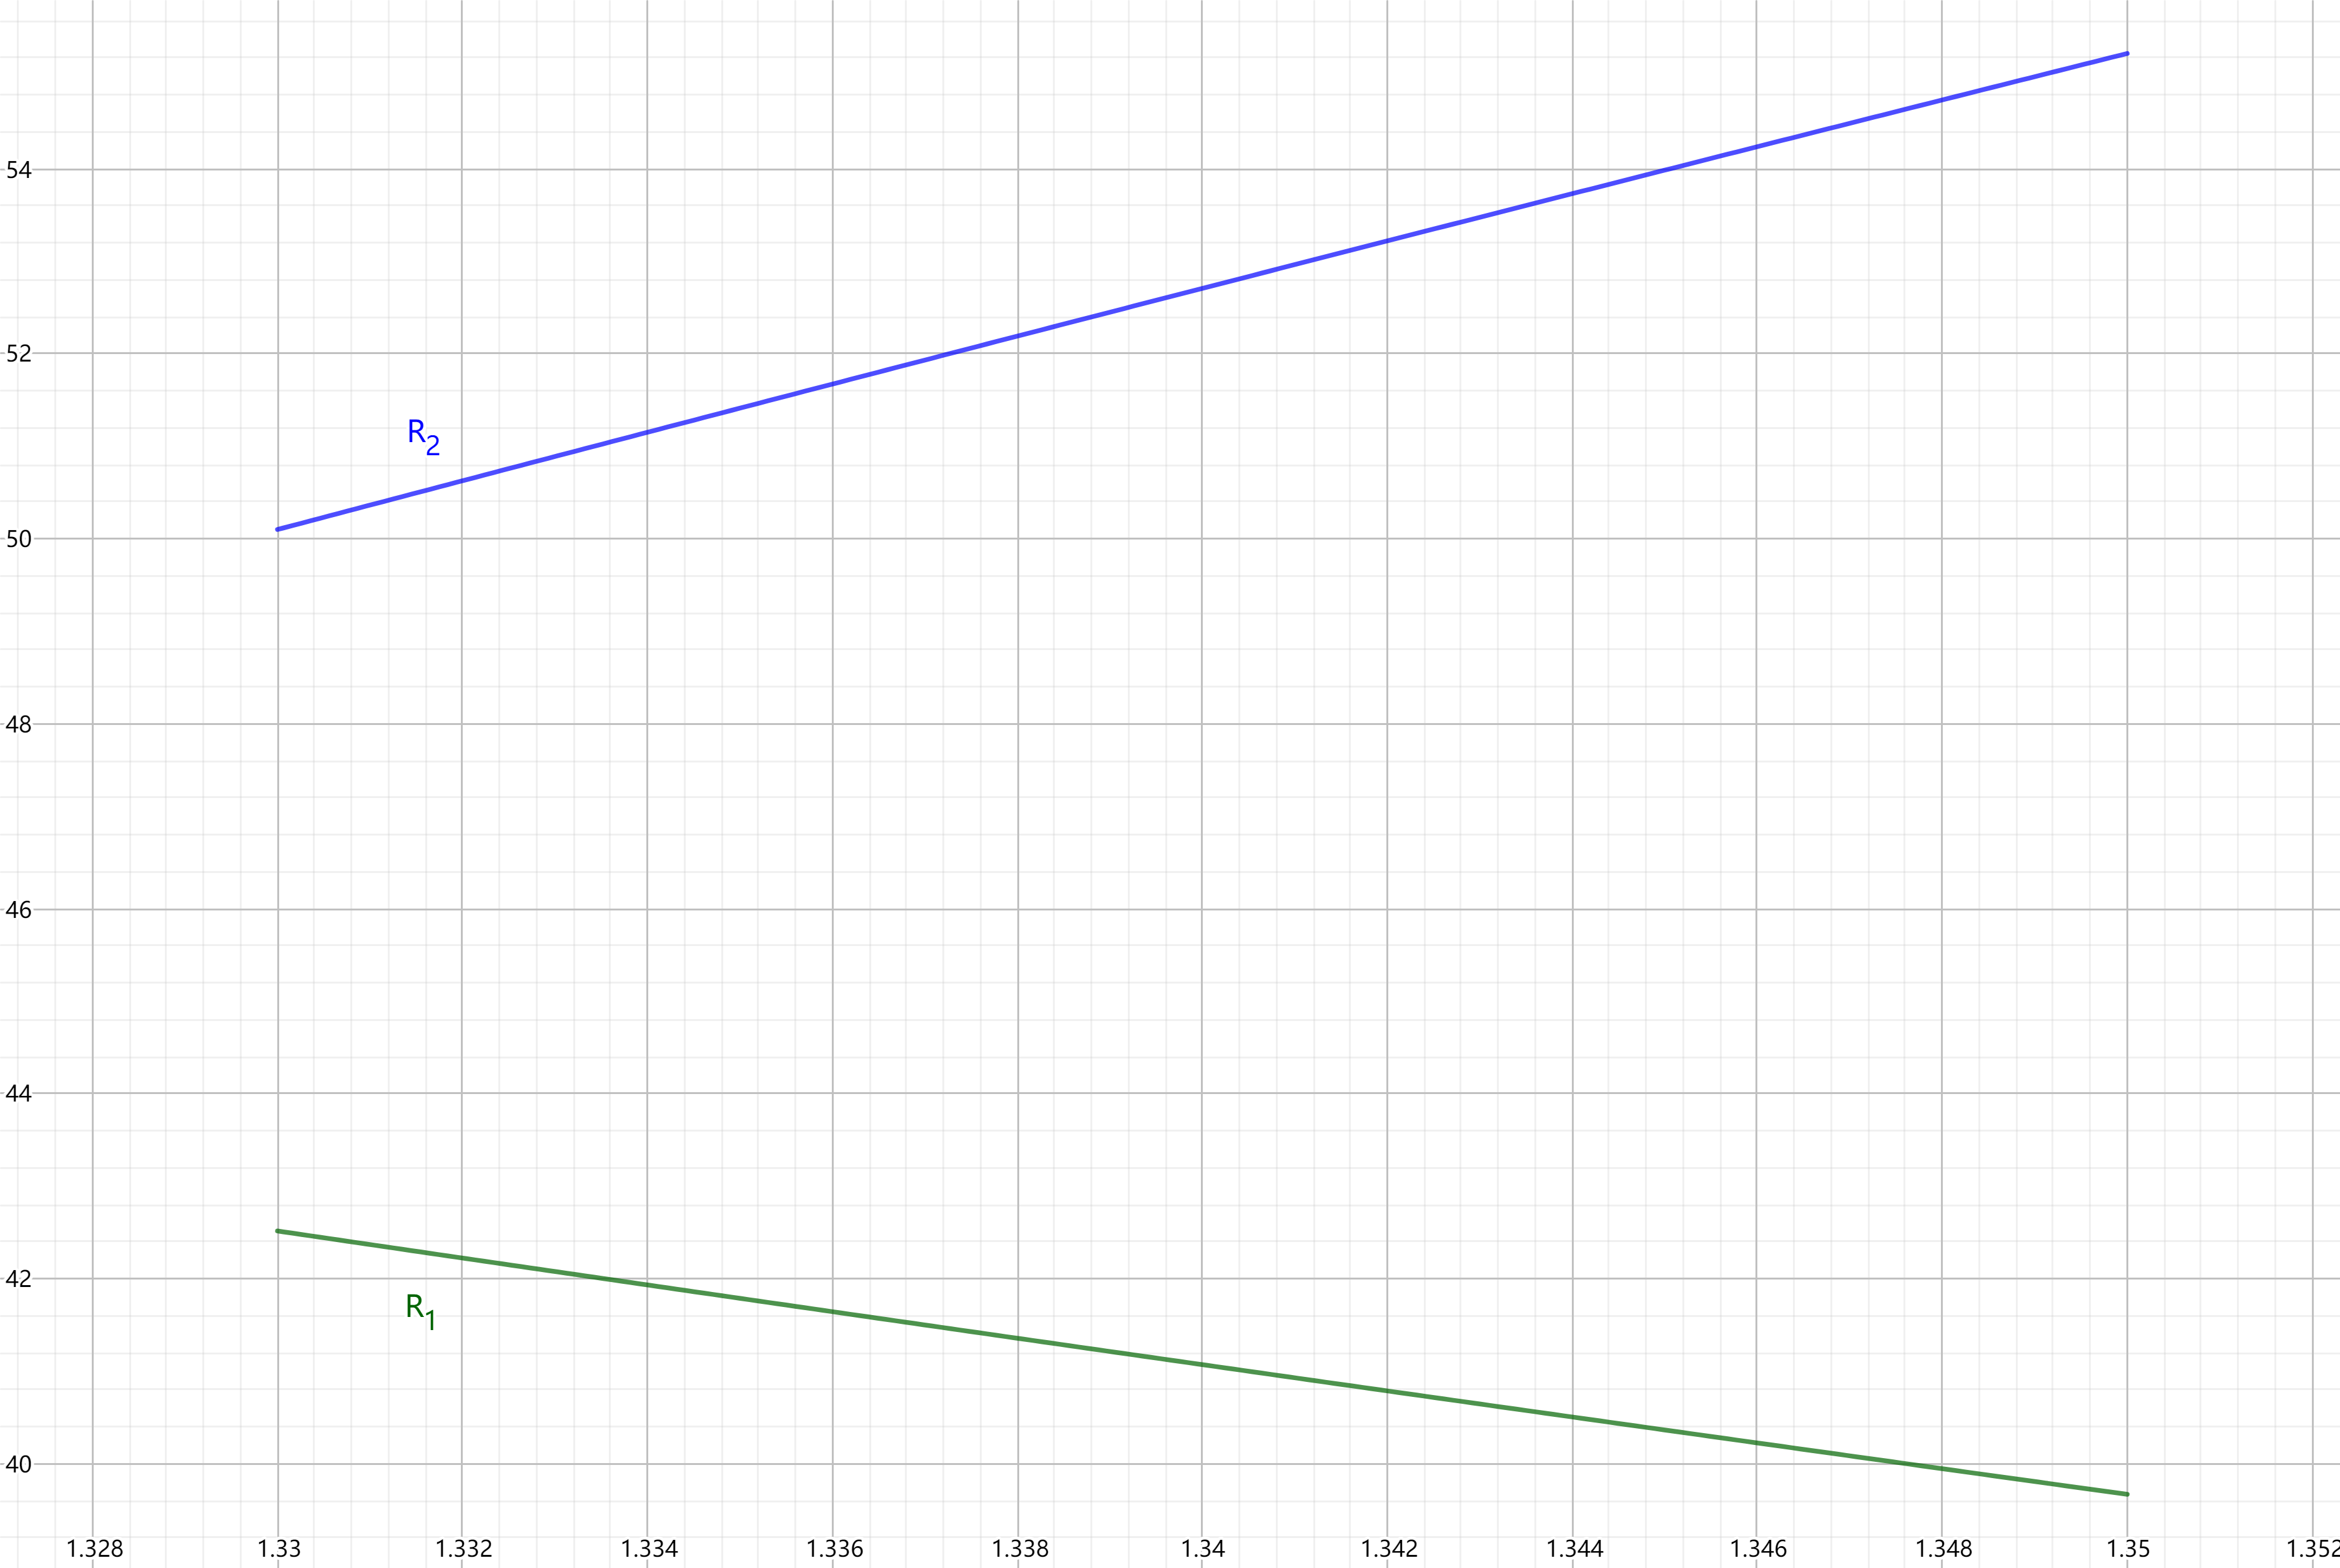
\includegraphics[scale=0.14]{微信图片_20221113175356}
   \caption[图6]{彩虹角R(角度制)-折射系数k}\label{fig-图6}
   \end{figure}
\nocite{*}
\bibliography{Task3}
\end{document}
